\documentclass{article}

\usepackage{tikz}
\usetikzlibrary{positioning}
\usetikzlibrary{fit}
\usetikzlibrary{calc}
\usetikzlibrary{shapes.geometric}
\usetikzlibrary{arrows.meta}
\usetikzlibrary{external}
\tikzexternalize

% Use the following line for the initial blind version submitted for review:
\definecolor{draculabg}      {RGB} {40,   42,   54}
\definecolor{draculacl}      {RGB} {68,   71,   90}
\definecolor{draculafg}      {RGB} {248,  248,  242}
\definecolor{draculacomment} {RGB} {98,   114,  164}
\definecolor{draculacyan}    {RGB} {139,  233,  253}
\definecolor{draculagreen}   {RGB} {80,   250,  123}
\definecolor{draculaorange}  {RGB} {255,  184,  108}
\definecolor{draculapink}    {RGB} {255,  121,  198}
\definecolor{draculapurple}  {RGB} {189,  147,  249}
\definecolor{draculared}     {RGB} {255,  85,   85}
\definecolor{draculayellow}  {RGB} {241,  250,  140}

\color{draculafg}

\begin{document}
\begin{figure}
	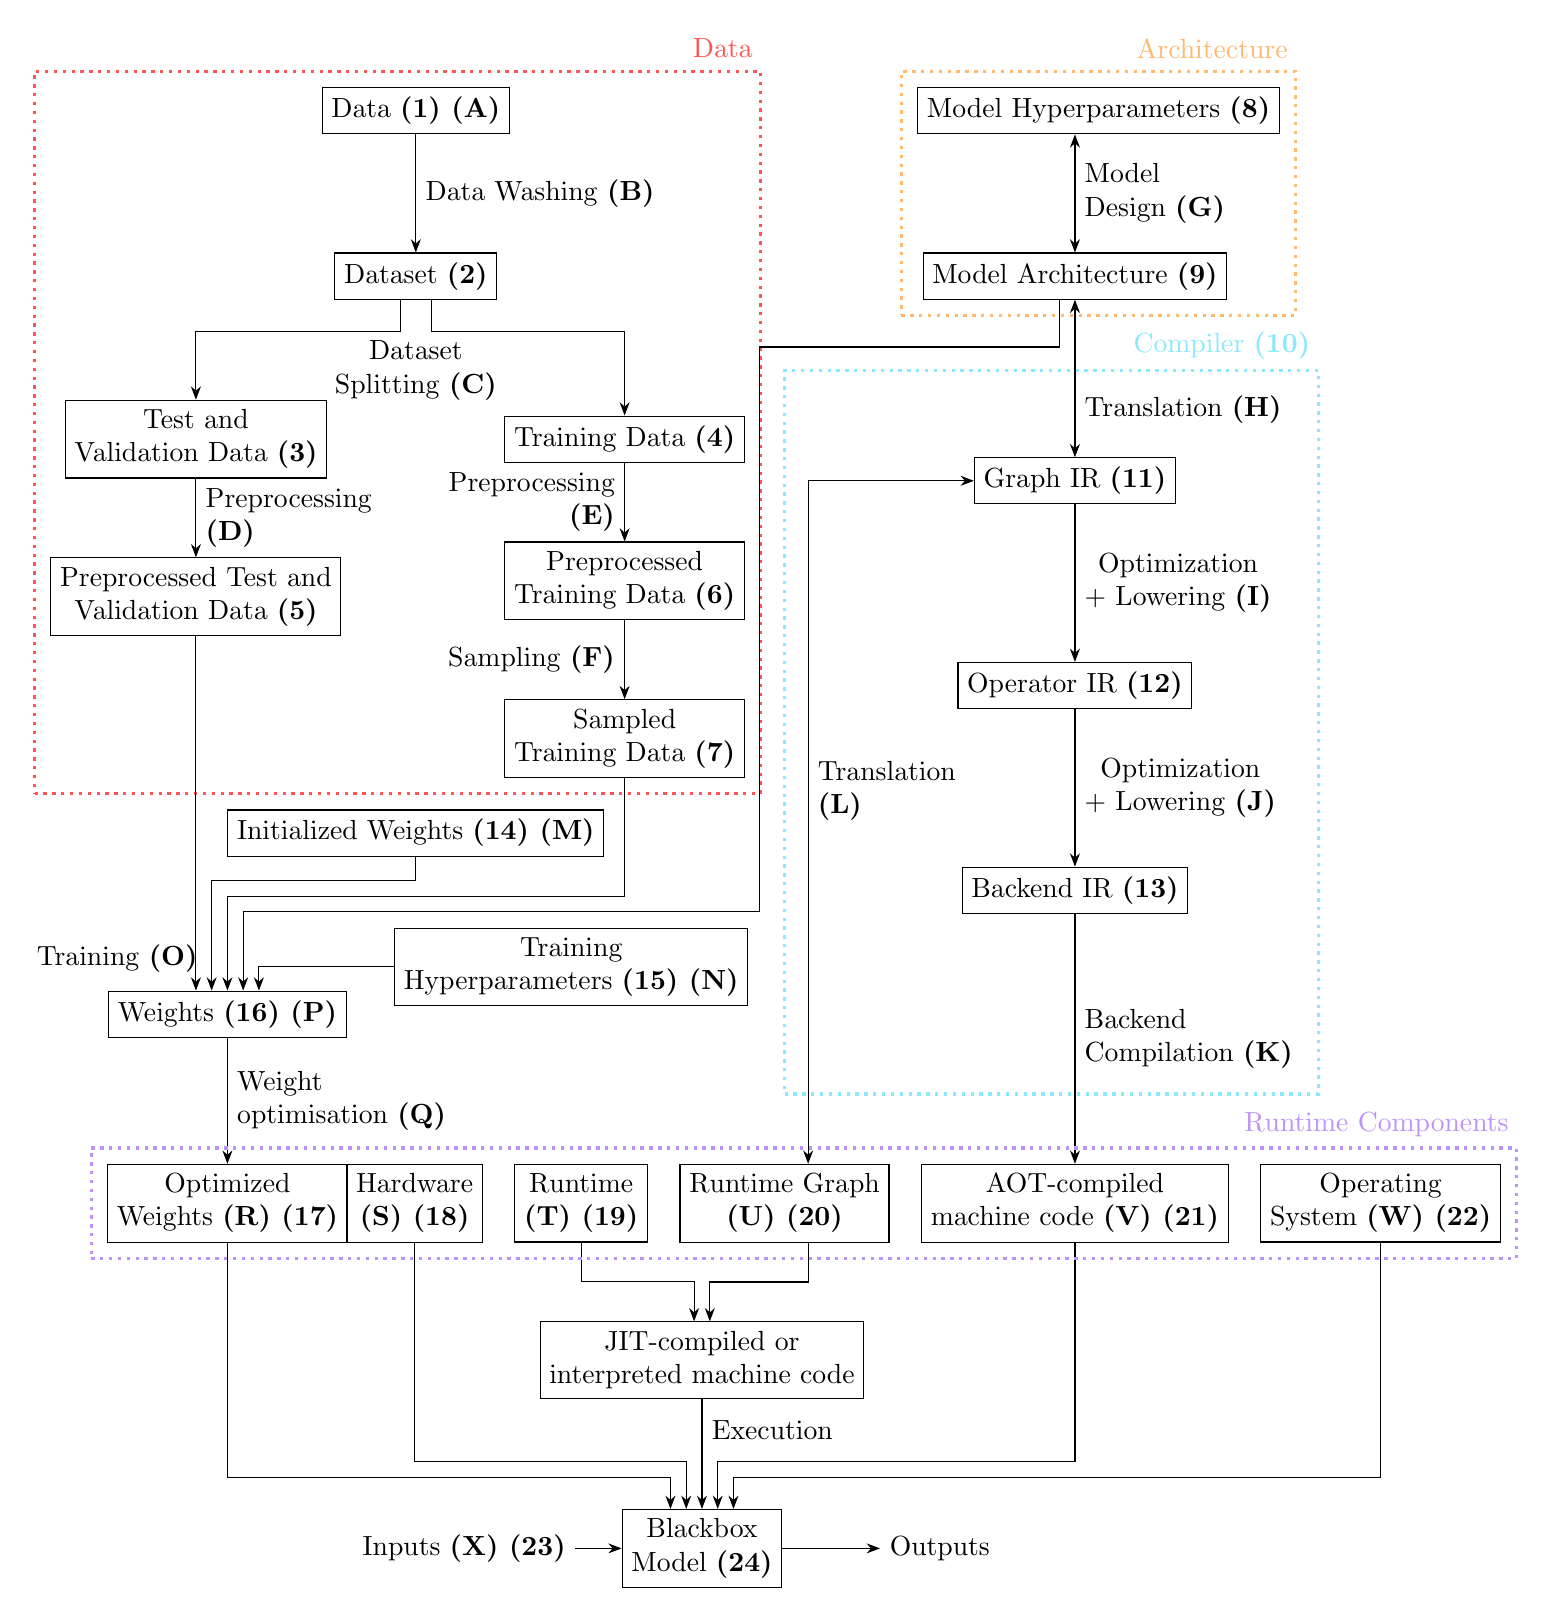
\begin{tikzpicture}[node distance=10mm, minimum height=1.5em, >={Stealth[scale=1]}]
	\node[draw]                                              (Hyperparameters)  {Model Hyperparameters \textbf{(8)}};
	\node[draw, xshift=-3mm, below=15mm of Hyperparameters]  (Arch)             {Model Architecture \textbf{(9)}};
	\node[draw, left=54mm of Arch]                           (Dataset)          {Dataset \textbf{(2)}};
	%\node[draw, left=37mm of Arch]                           (Dataset)          {Dataset \textbf{(2)}};

	\node[below=15mm of Dataset]  (helper1)  {};

	\node[draw, above=15mm of Dataset]               (Data)              {Data \textbf{(1) (A)}};
	\node[draw, right=10mm of helper1]               (TrainData)         {Training Data \textbf{(4)}};
	\node[draw, left=10mm of helper1, align=center]  (ValData) {Test and\\Validation Data \textbf{(3)}};
	\node[draw, below=of ValData, align=center]      (PPValData)         {Preprocessed Test and \\Validation Data \textbf{(5)}};
	\node[draw, below=of TrainData, align=center]    (PPTrainData)       {Preprocessed\\Training Data \textbf{(6)}};
	\node[draw, below=of PPTrainData, align=center]  (SampledTrainData)  {Sampled\\Training Data \textbf{(7)}};

	\draw[->] (Data) -- (Dataset) node [midway, right, align=left] (Washing) {Data Washing \textbf{(B)}};
	\draw[->]
		   ($(Dataset.south) - (2mm, 0mm)$)
		|- ($(Dataset.south) - (2mm, 4mm)$)
		-| (ValData);

	\node [below=4mm of Dataset, align=center] (Split) {Dataset\\Splitting \textbf{(C)}};

	\draw[->]
		   ($(Dataset.south) + (2mm, 0mm)$)
		|- ($(Dataset.south) + (2mm, -4mm)$)
		-| (TrainData);

	\draw[->] (TrainData) -- (PPTrainData) node[midway, left, align=right] (Preprocessing) {Preprocessing\\\textbf{(E)}};
	\draw[->] (PPTrainData) -- (SampledTrainData) node[midway, left] (Sampling) {Sampling \textbf{(F)}};

	\node[draw] (Weights) at ($(PPValData|-SampledTrainData) + (4mm, -35mm)$)
		{Weights \textbf{(16) (P)}};

	\node[draw, below=16mm of Weights, align=center] (OptWeights)
		{Optimized\\Weights \textbf{(R) (17)}};
	\node[draw]  (Init) at ($(Weights.north-|Dataset) + (0mm, 20mm)$)
		{Initialized Weights \textbf{(14) (M)}};

	\node[draw, right=6mm of Weights, yshift=6mm, align=center]
	(THyp) {Training\\Hyperparameters \textbf{(15) (N)}};

	\draw[->] (THyp.west) -| ($(Weights.north) + (4mm, 0)$);

	\draw[->]
		   (Init.south)
		-- ($(Init.south|-Weights.north) + (0mm, 14mm)$)
		-| ($(Weights.north) + (-2mm, 0mm)$);

	\node[draw, very thick, dotted, draculared, fit =
		(Data) (Dataset) (Dataset) (TrainData) (ValData)
		(PPTrainData) (PPValData) (SampledTrainData),
		inner sep=2mm] (DataBox) {};
	\node[draculared, anchor = south east] (DataLabel) at
		(DataBox.north-|DataBox.east) {Data};

	\draw[->] (SampledTrainData.south)
			|-  ($(Weights.north) + (0mm, 12mm)$)
			-|  ($(Weights.north) + (0mm, 0mm)$);



	%data
	%washing
	%dataset
	%training and validation
	%preprocess each
	%sample only training

	\draw[<->] ($(Hyperparameters.south) - (3mm, 0mm)$) -- (Arch) node
		[midway, right, align=left] (Design) {Model\\Design \textbf{(G)}};

	\node[right=9mm of Hyperparameters] (wallpusher) {};

	\node[draw, very thick, dotted, draculaorange, fit =
		(Hyperparameters) (Arch) (Design),
		inner sep=2mm] (ArchitectureBox) {};

	\node[draculaorange, anchor = south east] (ArchitectureLabel) at
		(ArchitectureBox.north-|ArchitectureBox.east) {Architecture};

	%\draw[<->]
		   %(Type)
		%|- ($(Arch.north) + (2mm, 3mm)$)
		%-| ($(Arch.north) + (2mm, 0)$);

	\node[draw, below=20mm of Arch] (Graph) {Graph IR \textbf{(11)}};

	%\draw[->] ($(Graph.east) + (0, 2mm)$) .. controls ($(Graph.east) + (4mm, 0mm)$) .. ($(Graph.east) - (0, 2mm)$);

	\draw[<->] (Arch) -- (Graph) node
		[midway, right, yshift=-4mm] (Trans)
		{Translation \textbf{(H)}};

	\node[draw, below=20mm of Graph] (Operator) {Operator IR \textbf{(12)}};
	\draw[->] (Graph) -- (Operator) node
		[midway,right,align=center] (GraphToOp)
		{Optimization\\+ Lowering \textbf{(I)}};

	\node[draw, below=20mm of Operator]  (Backend) {Backend IR \textbf{(13)}};
	\draw[->] (Operator) -- (Backend) node
		[midway,right,align=center] (OpToBackend)
		{Optimization\\+ Lowering \textbf{(J)}};

	\node[draw, align=center] (AOT) at (Backend|-OptWeights)
		{AOT-compiled\\machine code \textbf{(V) (21)}};

	\draw[->] (Backend) -- (AOT.north) node
		[midway, right,align=left] (BackendComp)
		{Backend\\Compilation \textbf{(K)}};

	\node (Training) at ($(Weights.north) + (-14mm, 4mm)$) {Training \textbf{(O)}};

	\draw[->] (ValData) -- (PPValData) node[midway, right, align=left] (ValPreprocessing) {Preprocessing\\\textbf{(D)}};
	\draw[->] (PPValData) -- ($(Weights.north) + (-4mm, 0mm)$);

	\node[left = 4mm of AOT, draw, align=center] (RTGraph)
		{Runtime Graph\\\textbf{(U) (20)}};

	\node[left = 4mm of RTGraph, draw, align=center] (Runtime)
		{Runtime\\\textbf{(T) (19)}};

	\draw[<->]
		   ($(Graph.west)$)
		   -- ($(Graph.west-|RTGraph.north) + (3mm, 0mm)$)
		   -- ($(RTGraph.north) + (3mm, 0mm)$)
		   node[midway, right, align=left, yshift=4mm] (GraphTrans)
	   {Translation\\\textbf{(L)}};

	\node[anchor=west, xshift=-1mm] (pusher) at (GraphTrans.west) {};

	\node[draw, very thick, dotted, draculacyan, fit =
		(Graph) (Trans) (Operator) (Backend) (GraphToOp)
		(OpToBackend) (BackendComp) (pusher),
		inner sep=2mm] (CompilerBox) {};

	\draw[->] ($(Arch.south)  - (2mm, 0)$)
		   -- ($(Arch.south)  - (2mm, 6mm)$)
		   -| ($(CompilerBox.west) + (-3mm, 0mm)$)
		   |- ($(Weights.north)  + (2mm, 10mm)$)
		   -- ($(Weights.north)  + (2mm, 0)$);


	\node[draculacyan, anchor = south east]
		(CompLabel) at (CompilerBox.north-|CompilerBox.east) {Compiler \textbf{(10)}};

	%\node[draw, align=center, right=4mm of OptWeights] (GPU) {Coprocessor\\(GPU) \textbf{(R) (20)}};
	\node[draw, align=center, left=4mm of Runtime] (Hardware)
		{Hardware\\ \textbf{(S) (18)}};

	\node[draw, align=center, anchor=north, yshift=-10mm] (JIT) at
		($(RTGraph.east|-RTGraph.south)!0.5!(Runtime.west|-Runtime.south)$)
		{JIT-compiled or\\interpreted machine code};

	\node[draw, below=14mm of JIT, align=center]
		(Model) {Blackbox\\Model \textbf{(24)}};

	\draw[->]
		($(RTGraph.south) + (3mm, 0mm)$)
		|- ($(RTGraph.south)!0.5!(JIT.north) + (0.5mm, 0mm)$)
		-| ($(JIT.north) + (1mm, 0mm)$);

	\draw[->]
		(Runtime.south)
		|- ($(Runtime.south)!0.5!(JIT.north) + (-0.5mm, 0mm)$)
		-| ($(JIT.north) + (-1mm, 0mm)$);

	\draw[->] (JIT) -- (Model) node[midway, right, yshift=3mm] (Execution) at (Model.north) {Execution};

	\node[draw, right=4mm of AOT, align=center] (OS) {Operating\\System \textbf{(W) (22)}};

	\draw[->]
		   (AOT.south)
		|- ($(Model.north) + (2mm, 6mm)$)
		-- ($(Model.north) + (2mm, 0mm)$);

	\draw[->]
		   (OS.south)
		|- ($(Model.north) + (4mm, 4mm)$)
		-- ($(Model.north) + (4mm, 0mm)$);

	\draw[->] (Weights) -- (OptWeights) node[midway, right,
	align=left] {Weight\\optimisation \textbf{(Q)}};

	\draw[->]
		   (OptWeights.south)
		|- ($(Model.north) + (-4mm, 4mm)$)
		-| ($(Model.north) + (-4mm, 0)$);

	%\draw[->]
		   %(GPU.south)
		%|- ($(Model.north) + (-2mm, 6mm)$)
		%-| ($(Model.north) + (-2mm, 0)$);

	\draw[->]
		   (Hardware.south)
		|- ($(Model.north) + (-2mm, 6mm)$)
		-| ($(Model.north) + (-2mm, 0)$);


	\node[draw, very thick, dotted, draculapurple, fit =
		(OptWeights) (Hardware) (AOT) (RTGraph) (Runtime) (OS),
		inner sep=2mm] (RuntimeBox) {};

	\node[draculapurple, anchor = south east, align=center] (RuntimeLabel) at
		(RuntimeBox.north-|RuntimeBox.east) {Runtime Components};


	\node  (Inputs)   at ($(Model.west) - (20mm, 0)$)  {Inputs
		\textbf{(X) (23)}};
	\node  (Outputs)  at ($(Model.east) + (20mm, 0)$)  {Outputs};

	\draw[->] (Inputs) -- (Model);
	\draw[->] (Model) -- (Outputs);

\end{tikzpicture}

\end{figure}
\end{document}

